\section{Aplicación de ejemplo}

Para comprender mejor esta problemática veamos un ejemplo. Supongamos una simple
aplicación bancaria, donde los clientes de un banco pueden transferir dinero de
una cuenta a otra. Al realizar un transferencia, hay que extraer el monto
indicado de la primera cuenta, y depositarlo en la segunda. Estas dos
operaciones pueden tener errores, como por ejemplo, extraer un monto mayor al
saldo, o depositar mas cantidad de la maxima permitida.

La  figura \ref{example} muestra el diagrama de la aplicación de
ejemplo

	\begin{figure}[h]
		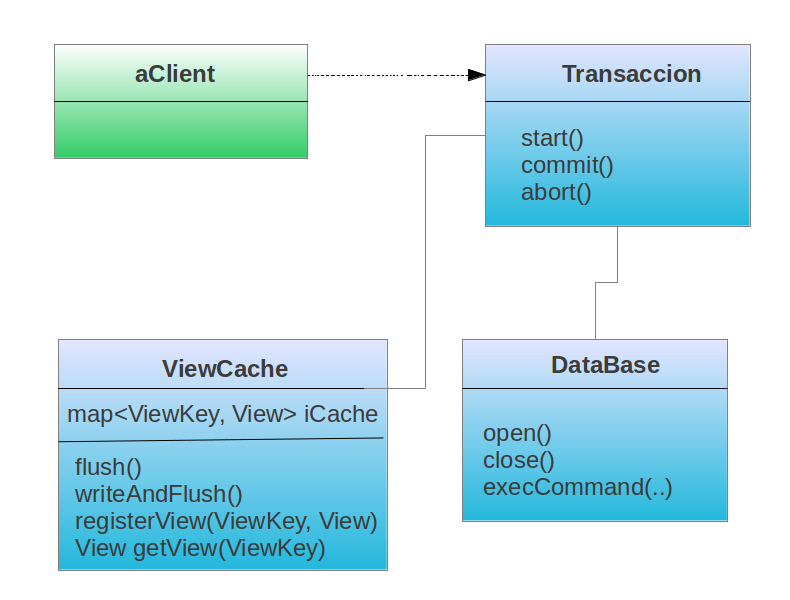
\includegraphics{img/objectTransaction}
		\caption{Diagrama UML de la aplicación de ejemplo}
		\label{example}
	\end{figure}	


El sistema me permite 

\section{Nuestra herramienta: }

Con el propósito de cumplir el objetivo detallado en la Sección
\ref{sec:Objetivo} y llevándolo a cabo con la solución propuesta en la  la
Sección \ref{sec:Solucion}, se desarrolló dos conceptos \emph{Pure Objects
Observable} (POO)  para atacar a la problemática de la observabilidad y
\emph{Pure Object Transaction} (POT) para atacar a la problematica
transaccional.

\medskip  

Se evaluaron dos frameworks para resolver nuestro problema. Uno es Javassist y
el otro AspectJ. \cite{KiczalesHHKPG01}

\medskip 

Se utilizó Javassist porque es independiente al usuario, en cambio si utilizamos
AspectJ obligamos al usuario a el compilador del código. 

\medskip 

Ya que Javassist es muy de bajo nivel, y trabaja a nivel de \emph{bytecode},
trajabar con el es complicado y el codigo se hace intendible. Por eso se
desrrollo una herramienta llamada \emph{ Aspect for Pure Object} (APO), que es 
una abstracción del Framework Javassist, que permite fácilmente implementar un
aspecto, y aplicarselo a un grupo de objetos.

\comment{Hay ciertos parametros en la aplicación que son configurables. Para
ello hay que editar el archivo \emph{framework-config.properties}}.

\medskip 

Utilizando \emph{APO} se implementaron los dos aspectos diferentes:

	\subsection{Aspecto Transaccional (POO)} 
		Esta basado en una implementación
		hecha por Nicolás Passerini y Javier Fernandes.
		 
		Utilizando la programación orientada a aspectos, intercepta todas las lecturas
		y escrituras de los \emph{fields}. Insertando código al momento de la carga de
		la clase.
		Se remplaza el acceso al field, tanto de lectura como escritura, y se lo delega
		al ObjectTransactionManager, donde se guarda la información en una estructura
		[objeto, [Field, Valor]].
		
		\medskip
		
		El contexto de la transacción esta asociado a un solo \emph{tread}. Esto
		permite manejar la concurrencia en el acceso a la información de los objetos. 
		Soportando transacciones anidadas, donde cada transacción hija hereda el estado
		de su padre, y al momento de hacer el \emph{commit} en la sub-transacción, sus
		cambios son impactados en la transacción padre.
		Por esta forma de implementación, la identidad del objeto se mantiene, ya que
		el objeto no se modifica ni se clona, solo se cambia el acceso a sus fields.
		
		Para agregarle este aspecto a una clase se utiliza la \emph{Annotation}
		\emph{Transactional }
		
			\begin{lstlisting} 
				@Transactional
				public class Client extends Entity {
				}
			\end{lstlisting}

	\subsection{ Aspecto Observable}
			
		En su implementación interna lo que hace el aspecto es agregar un \emph{field
		changeSupport} del tipo \emph{<<PropertySupport>>} al objeto que se va a
		convertir en Observable. Pero su implememtacion se optiene del el archivo de
		configuracion con la \emph{key: framework.aop.poo.changeSupport}.
		Luego se agrega métodos para completar su objetivo.
		El primero es el \emph{firePropertyChange} que es el que notifica a los
		Observadores que una propiedad ha cambiado.	Luego le agregamos
		\emph{addPropertyChangeListener} y \emph{removePropertyChangeListener} para
		poder agregar y remover Observadores para que escuchen sus cambios.
		
		Para agregarle este aspecto a una clase se utiliza la \emph{Annotation}
		\emph{Observable}
		
			\begin{lstlisting} 
				@Observable
				public class Client extends Entity {
				}
			\end{lstlisting}
		


\subsection{Integración de ambos aspectos } 
	Framework me permite poder tener uno u otro , o
	ambos aspecto. Se puede poner los dos \emph{Annotation} \emph{Observable} y
	\emph{Transactional} como vimos previamente, o ponerle uno solo. 
	
	\begin{lstlisting} 
		@TransactionalAndObservable
		public class Client extends Entity {
		}
	\end{lstlisting}
	
	
	
\subsection{Integración de aspectos con el Arena}
	En Arena se integró los dos aspectos, el Observable y el transaccional, con el
	fin de que los objetos de dominio sean puros, y que no tengan la noción de
	eventos, ni transacciones, y así poder bindearlos con los componentes de de la
	interfaz gráfica. Y al cancelar la edición poder revertir los cambios
	transparéntenme.
	
	Para ello se tubo que asociar una transacción con una ventana, en el caso mas
	especifico con la clase \emph{TransactionalDialog}. A su vez también tenemos
	vinculado los eventos del dominio junto con la ventana y la transacción.
	Se implemento tres niveles de aislamiento de los eventos,  \emph{Fire All},
	\emph{Fire Committed} y \emph{Fire olnly in my transaction};
	
	\begin{description}
		\item[\emph{Fire All}] Todos los eventos disparados por el dominio son
		escuchados, sin importar si están en una transacción.
	
		\item[\emph{Fire Committed}] Solo se escucha los eventos de las transacciones
			comiteadas
		
		\item[\emph{Fire olnly in my transaction}] solo se escucha los eventos que
			ocurren dentro de su translación.
	
	 \end{description}
	 
	 \medskip
	 
	\subsubsection{Monitor de Transacciones}
	
	 Con arena también se desarrolló un {\bf Monitor de Transacciones}, que me
	 muestra el estado actual de la transacción, incluyendo las transacciones
	 anidadas. Mostrandome los objetos afectados por la transacción y que
	 propiedades se modificaron.
	 
	 
 

	
\subsection{Buscar un  titulo}
La implementación de la integración en el arena se realizó con Scala, agregando
mejora al Arena como: Árboles, Listas \ldots \ldots \ldots. 
	
	
Contar que esta publicado, con la licencia y blah

Test de los aspectos


